\chapter{System morphology}
\label{sec:morphology}

In this section we describe how to specify the morphology of the system. We will use DCV2T as an example.

\section{Single molecule}

\begin{wrapfigure}{ht}{0.5\linewidth}
\centering
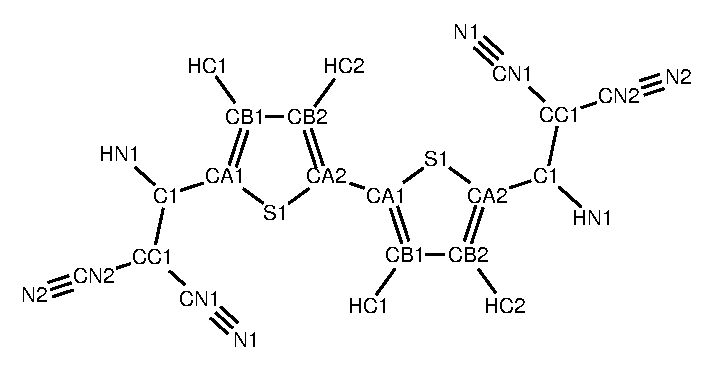
\includegraphics[width=0.9\linewidth]{./fig/chemical_structure/dcv2t_atom_types}
\caption{\small Atom types of DCV2T. The molecule consists of two building blocks (residues): thiophene (THI) and dicyanovinyl (NIT). }
\label{fig:dcv2t_at}
\end{wrapfigure}

%\clearpage
The structure of DCV2T, together with atom type definitions, is shown in fig.~\ref{fig:dcv2t_at}. DCV2T is a typical donor-acceptor-type molecule, with two electron-donating thiophene and two electron-withdrawing dicyanovinyl groups. The pdb file which contains residue types, residue numbering, atom names, atom types, and atom coordinates is shown below. In its ground state the molecule is practically planar. 

\section{Simulation box}
An amorphous morphology was obtained by quenching the 512 DCV2T molecules after equilibrating the system above the glass transition temperature. What we will need is a snapshot out of the trajectory and the topology file describing the system (all in GROMACS format).

\clearpage
\lstinputlisting[
  basicstyle=\ttfamily\footnotesize,
  frame=lines,
  identifierstyle=\color{red},
  keywordstyle=\color{blue},
  showstringspaces=false,
 label=list:pdb, 
 morekeywords={HETATM,THI,NIT},
 caption={pdb file of DCV2T}]%
{./fig/chemical_structure/dcv2t.pdb}

%\VerbatimInput[%
%frame=lines,
%framesep=4mm,
%label=\fbox{pdb file of DCV2T}, 
%framerule=0.5mm,
%rulecolor=\color{red},
%baselinestretch=1,
%fontsize=\footnotesize%,
%numbers=left
%]%
%{./fig/chemical_structure/dcv2t.pdb}
